\documentclass[usenames,dvipsnames,notes]{beamer}
\usepackage{ifthen}
\usepackage{xcolor}
\usepackage{pgfplots}
\usepackage{amsmath}
\usepackage{centernot}
\usepackage{pifont}
\usepackage{tabularx}
\usepackage{makecell}
\usepackage{cuted}
\usepackage{booktabs}
\usepackage{array}
\usepackage{setspace}
\usepackage{CJKutf8}
\usepackage{textcomp}


%\usepackage{pgfpages}
%\setbeameroption{show notes on second screen}

\pgfplotsset{compat=1.17}

\input ../beamer-style
\input ../std-macros
\input ../macros

\AtBeginSection[]
{
    \begin{frame}
        \frametitle{Table of Contents}
        \tableofcontents[currentsection]
    \end{frame}
}



\title[CSCI-GA.2590]{Introduction}
\author[He He]{He He
}
\institute[NYU]{New York University}
\date{\today}

%\includeonly{conclusion}
%\includeonlyframes{current}

\begin{document}

\begin{frame}
\titlepage
\end{frame}

\begin{frame}
{Logistics}
            \begin{tikzpicture}
                \node[circle,draw,inner sep=0.7cm,label=below:He He ,
                    path picture={
                        \node at (path picture bounding box.center){
                            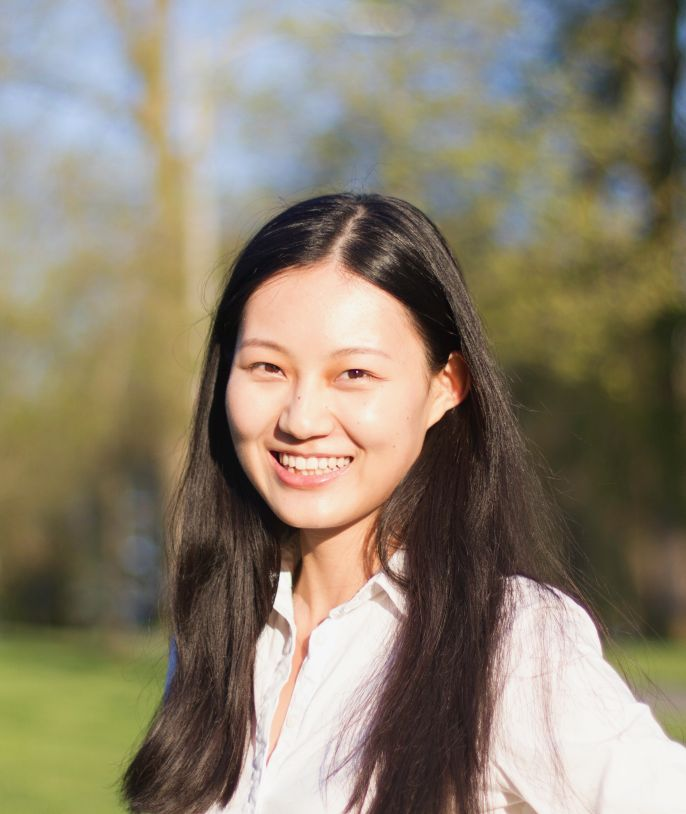
\includegraphics[width=4cm]{figures/hehe.jpg}
                        };
                    }] at(-3,0){};
                \node[circle,draw,inner sep=0.7cm,label=below:Gaomin Wu,
                    path picture={
                        \node at (-0.2, -0.3){
                            \includegraphics[width=4cm]{figures/gaomin.jpg}
                        };
                    }](gaomin) at (0, 0) {};
                \node[circle,draw,inner sep=0.7cm,label=below:Shivesh Ganju,
                    path picture={
                        \node at (path picture bounding box.center){
                            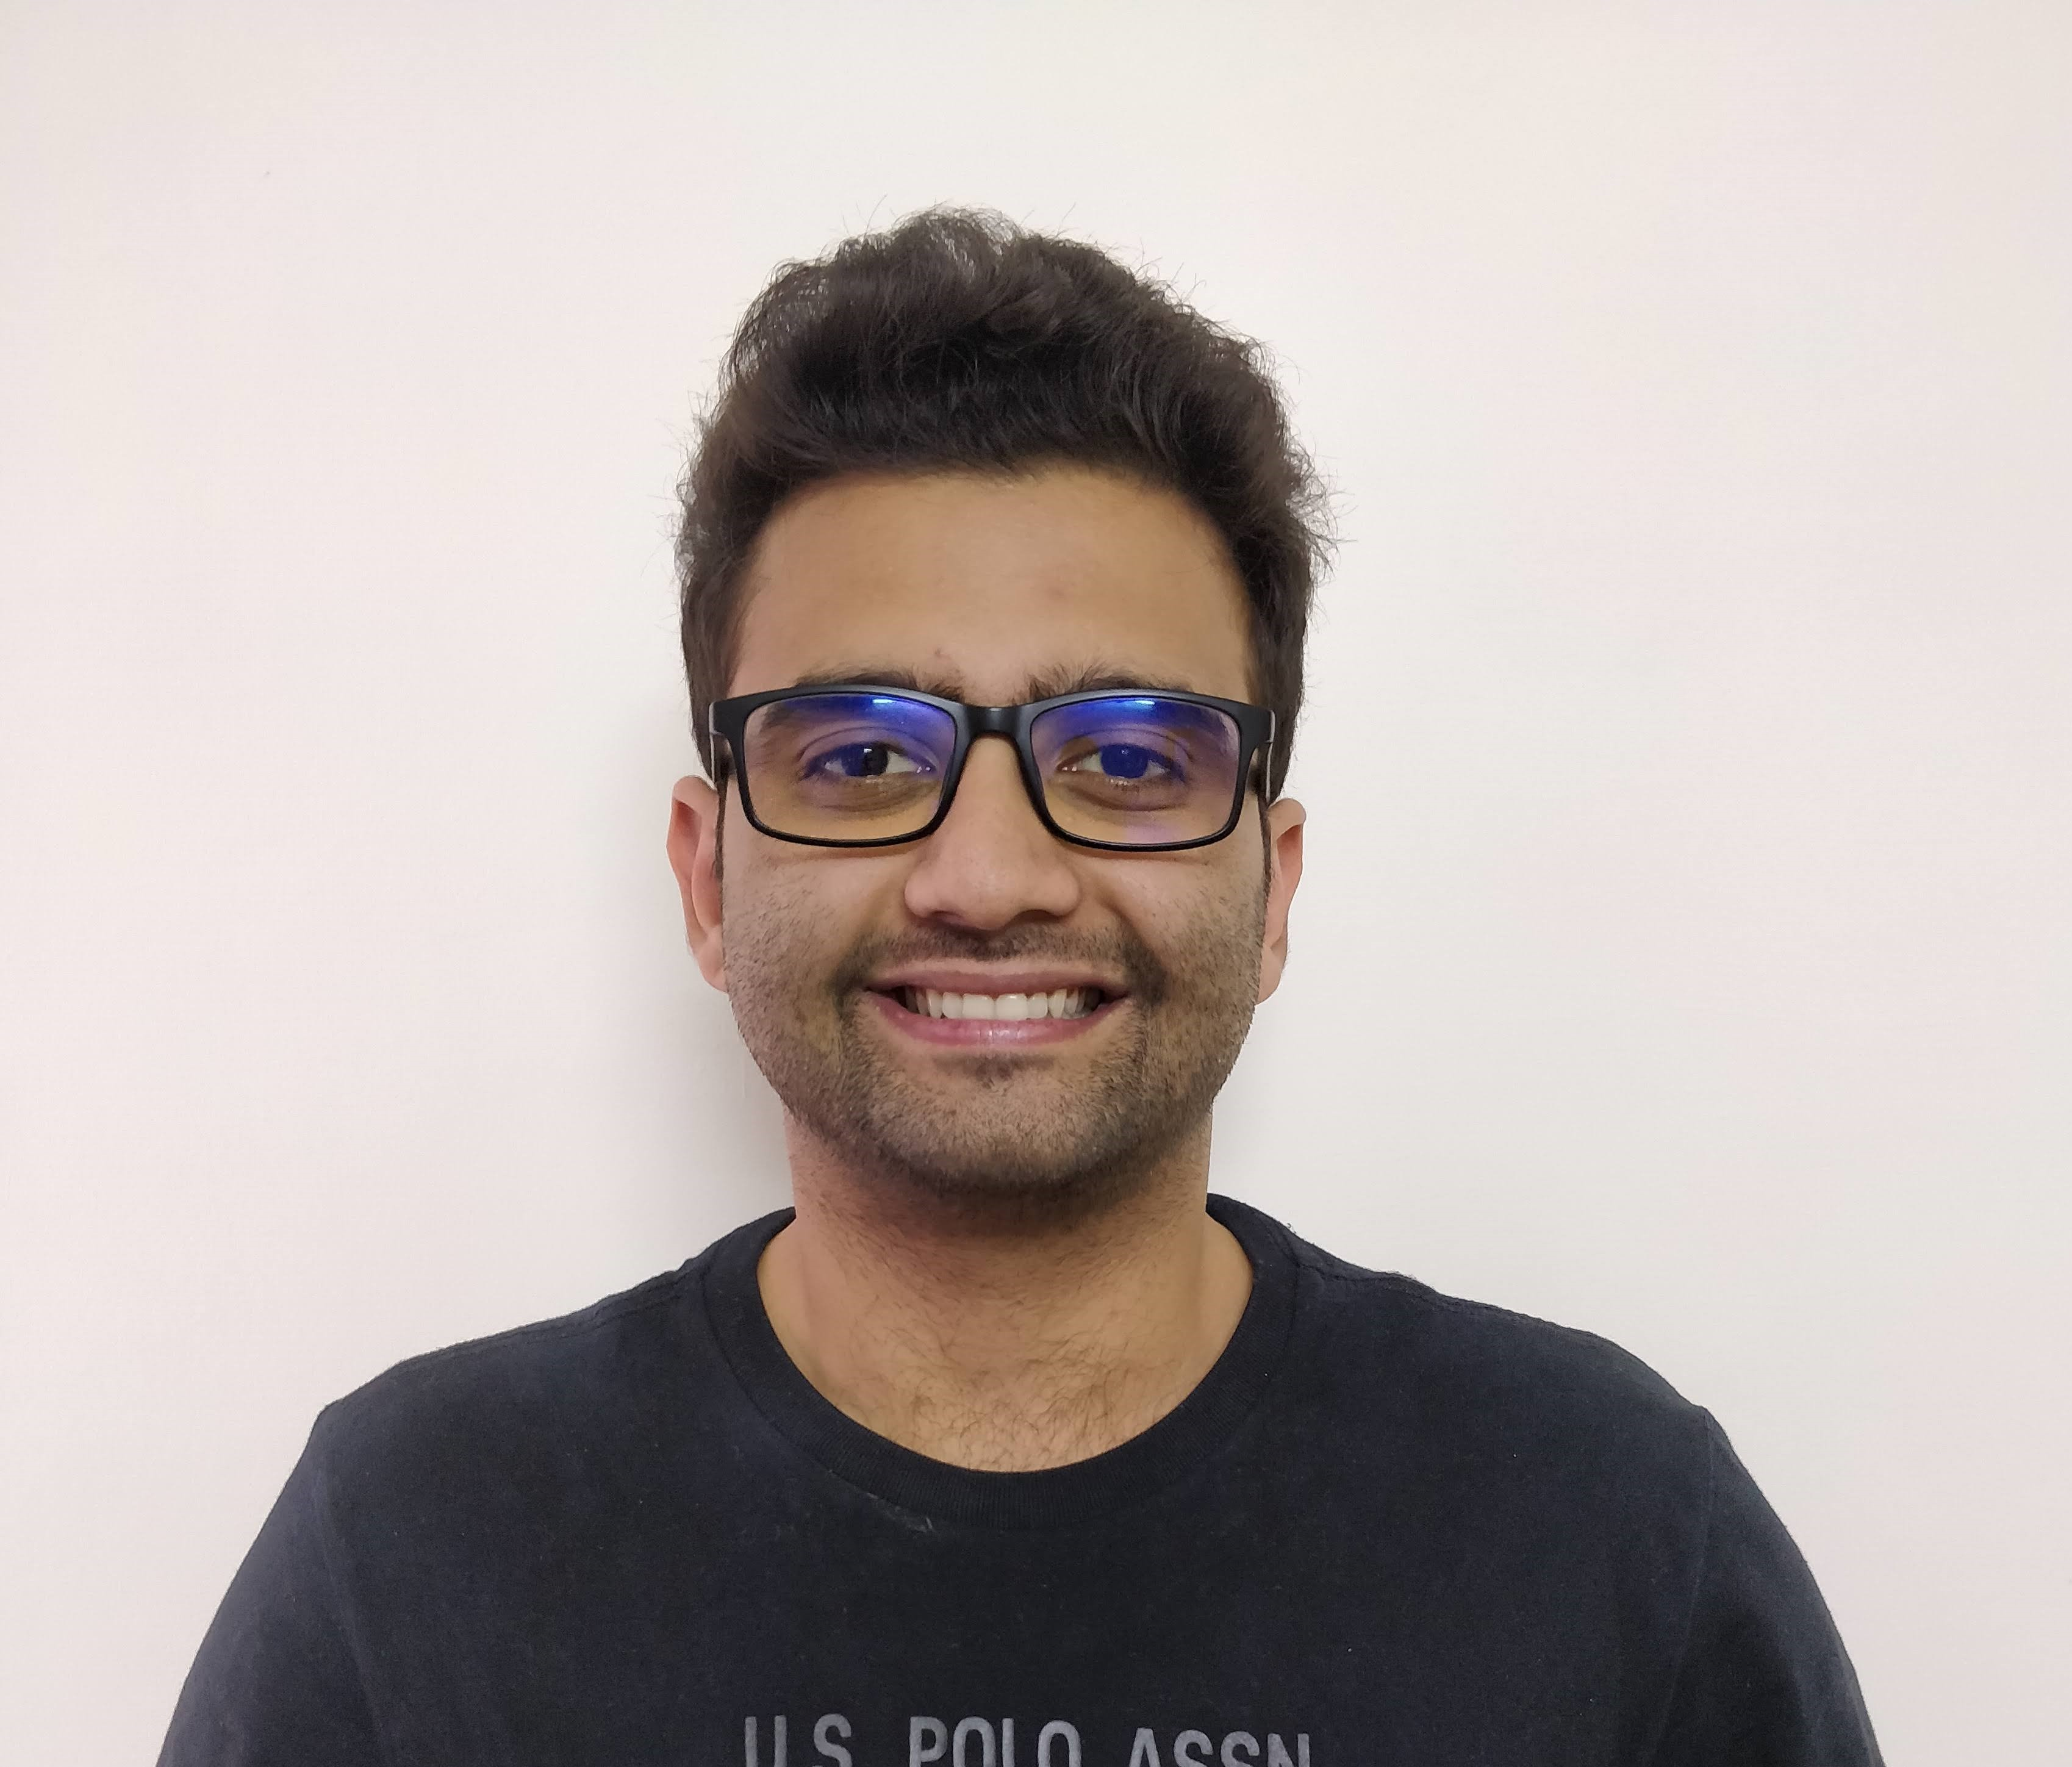
\includegraphics[width=4cm]{figures/shivesh.jpg}
                        };
                    }](shivesh) at (3, 0) {};
                \node[circle,draw,inner sep=0.7cm,label=below:Gauri Dhawan,
                    path picture={
                        \node at (0.7, -0.9){
                            
\includegraphics[width=4cm]{figures/gauri.jpg}
                        };
                    }](gauri) at (6, 0) {};
            \end{tikzpicture}
            \bigskip
    \begin{itemize}
        \item Best way to communicate: Piazza (\textcolor{red}{remember to sign up}).
        \item Lectures and office hours will be online (sadly).
        \item Let us know if you have accessibility needs.
    \end{itemize}
\end{frame}

\begin{frame}
    {What you'll be able to do by the end of this course}
    \begin{itemize}
        \itemsep1em
        \item Understand the core problems and challenges in NLP
        \item Formalize tasks as statistical learning problems
        \item Have a toolbox for solving different families of NLP problems
        \item Gain hands-on experience in building NLP systems
    \end{itemize}
\end{frame}

\begin{frame}
    {What we expect you to know}
    \begin{itemize}
        \itemsep1em
        \item \textbf{Linear algebra}: vector, dot product, gradient computation etc.
        \item \textbf{Probability and statistics}: conditional probability, expectation, Bayes rule etc.
        \item \textbf{Basic machine learning}: loss function, gradient descent etc.
        \item \textbf{Programming}: read and write Python code, use Numpy (and MXNet)
    \end{itemize}
\end{frame}

\section{A brief history}
\begin{frame}
    {Products powered by NLP technologies}
    \begin{tikzpicture}
        \node (translation) {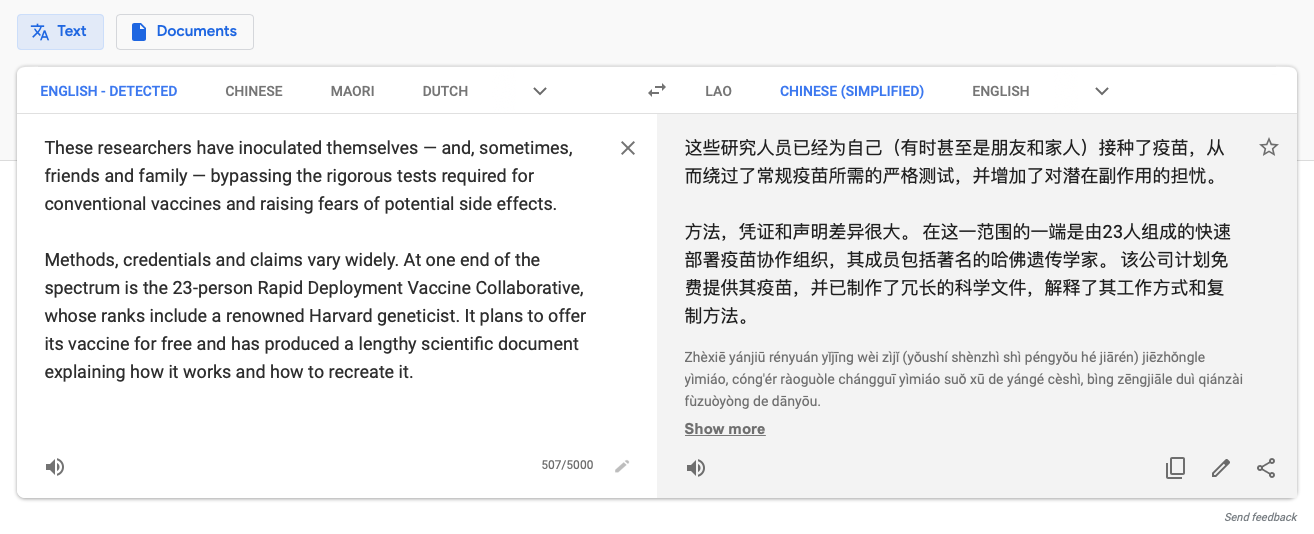
\includegraphics[width=10cm]{figures/google-translate}};
        \node (qa) [below= of translation, anchor=north east, yshift=3em]{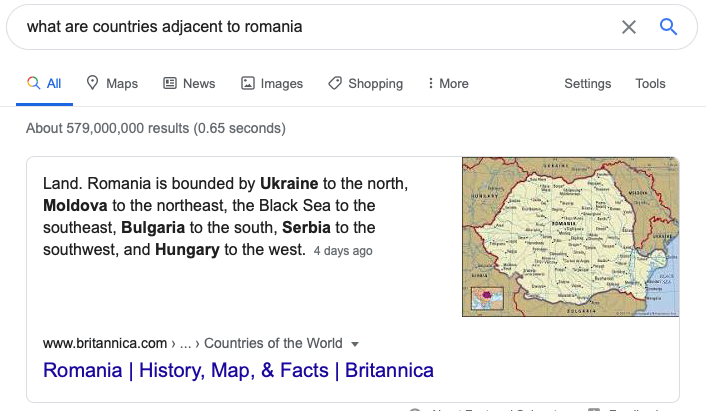
\includegraphics[width=5cm]{figures/search-qa}};
        \node [right= of qa]{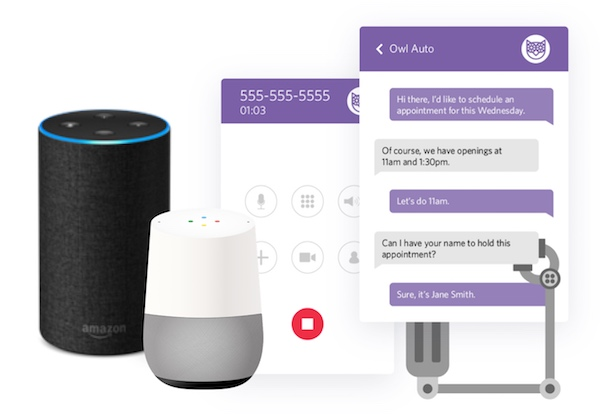
\includegraphics[width=5cm]{figures/alexa}};
    \end{tikzpicture}
\end{frame}

\begin{frame}
    {The imitation game}
    \begin{figure}
        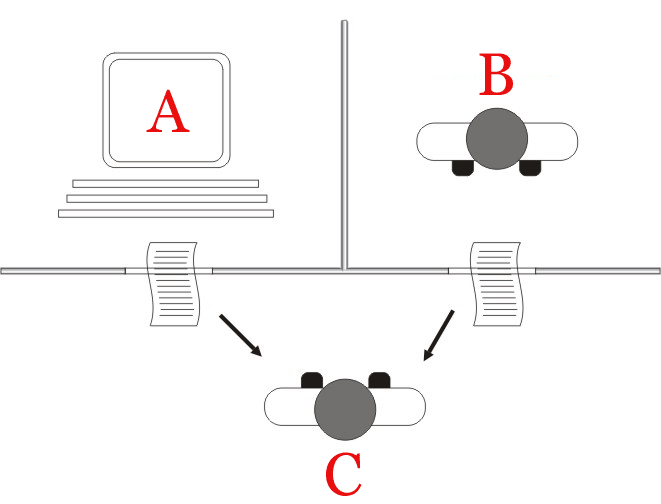
\includegraphics[height=3cm]{figures/turing-test}
    \end{figure}

    \nl{I believe that in about \emph{fifty years'} time it will be possible to programme computers, with a \emph{storage capacity of about $10^9$}, to make them play the imitation game so well that an average interrogator will not have more than 70 percent chance of making the right identification after five minutes of questioning.} Turing (1950)
    %I believe that at the end of the century the use of words and general educated opinion will have altered so much that one will be able to speak of machines thinking without expecting to be contradicted.'' 

\end{frame}

\begin{frame}
    {The Georgetown-IBM experiment}
    \begin{itemize}
        \item The program:\\
            \begin{center}
            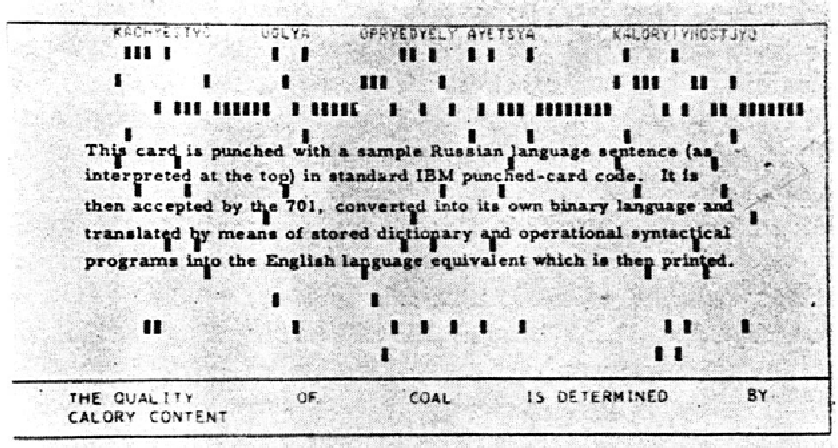
\includegraphics[height=3cm]{figures/ibm-experiment}
            \end{center}
        \item 250 words
        \item 6 grammar rules, e.g.\\
            ``If first code is 110, is third code associated with preceding complete word equal to 21? If so, reverse order of appearance of words in output (i.e., word carrying 21 should follow that carrying 110)---otherwise, retain order.''
    \end{itemize}
\end{frame}

\begin{frame}
    {ELIZA}
    \begin{itemize}
        \item Built by Joseph Weizenbaum at MIT in 1964 to demonstrate the \emph{superficiality} of human-machine communication.
        \item Surprisinly, people were convinced that ELIZA had human intelligence.
    \end{itemize}
    \bigskip
    \centering
    \begin{simpleblock}{}
    Human: Well, my boyfriend made me come here.\\
    ELIZA: Your boyfriend made you come here?\\
    Human: He says I'm depressed much of the time.\\
    ELIZA: I am sorry to hear you are depressed.\\
    Human: It's true. I'm unhappy.\\
    ELIZA: Do you think coming here will help you not to be unhappy?
    \end{simpleblock}
\end{frame}

\begin{frame}
    {SHRDLU}
    \begin{itemize}
        \item Built by Terry Winograd at MIT in 1968.
    \end{itemize}
    \begin{center}
    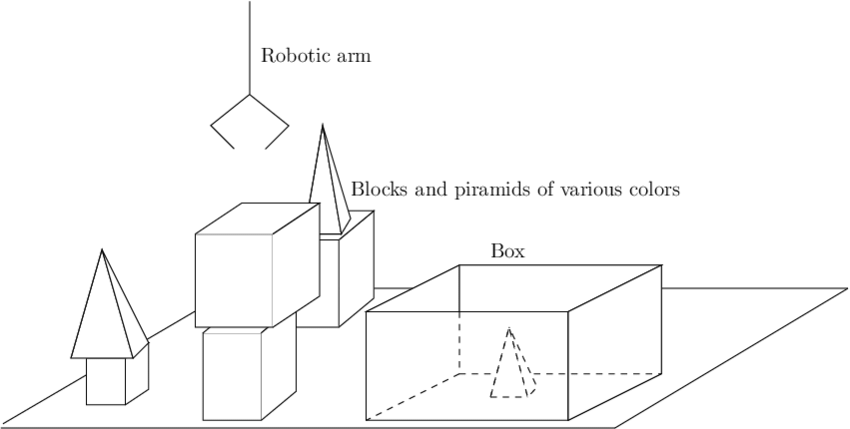
\includegraphics[height=3cm]{figures/shrdlu}
    \end{center}
    \begin{simpleblock}{}
        Person: Pick up a big red block.\\
Computer: OK.\\
Person: Grasp the pyramid.\\
Computer: I DON'T UNDERSTAND WHICH PYRAMID YOU MEAN.\\
Person (changing their mind): Find a block which is taller than the one you are holding and put it into the box.\\
Computer: BY "IT", I ASSUME YOU MEAN THE BLOCK WHICH IS TALLER THAN THE ONE I AM HOLDING.
    \end{simpleblock}
\end{frame}

\begin{frame}
    {Limitations of early systems}
    \begin{itemize}
        \itemsep1em
        \item Optimism in the 50's and 60's\\
            \nl{Within the very near future---much less than twenty-five years---we shall have the technical capability of substituting machines for any and all human functions in organizations.}
        \item Disappointing results due to
            \begin{itemize}
                \item \textbf{Limited computation}: hardware limitation 
                \item \textbf{Combinatorial explosion}: algorithms are intractable in realistic settings
                \item \textbf{Underestimated complexity}: ambiguity, commonsense knowledge etc.
            \end{itemize}
    \end{itemize}
\end{frame}

\begin{frame}
    {The rise of statistical learning in the 80's}
    \begin{itemize}
        \itemsep1em
        \item Notable progress in MT from IBM (neglected knowlege of linguistics).
        \item HMMs widely used for speech recognition.\\
            \nl{Every time I fire a linguist, the performance of the speech recognizer goes up.}---Frederick Jelinek.
        \item Machine learning is the main driving force of NLP today.
    \end{itemize}
\end{frame}

\section{Challenges in NLP}
\begin{frame}
    {Are we there yet?}
    Predictions are not robust to benign perturbations [Ribeiro+ 2020].
    \begin{figure}
        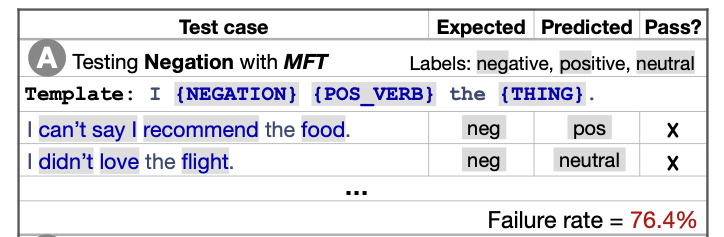
\includegraphics[width=10cm]{figures/checklist}
    \end{figure}
\end{frame}

\begin{frame}
    {Are we there yet?}
    MT systems are prone to gender-biased translation errors [Stanovsky+ 2019].
    \begin{figure}
        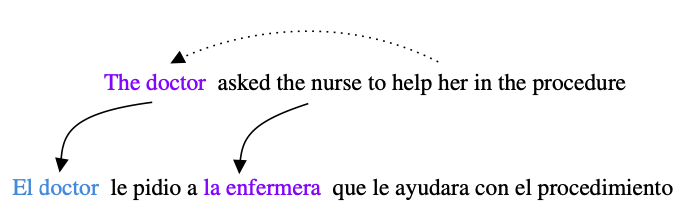
\includegraphics[width=10cm]{figures/gender-bias-example}
    \end{figure}
\end{frame}

\begin{frame}
    {Are we there yet?}
    QA models are easily distracted by irrelevant sentences [Jia+ 2017].
    \begin{figure}
        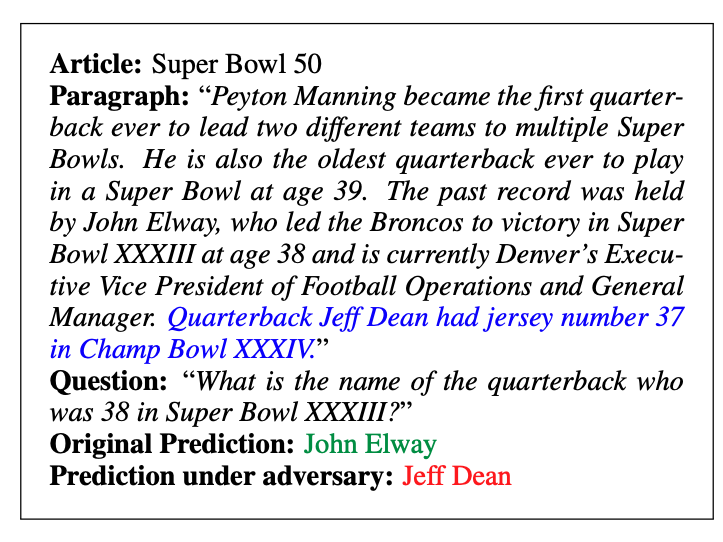
\includegraphics[height=6cm]{figures/qa-adv}
    \end{figure}
\end{frame}

\begin{frame}
    {Why is language hard?}
    \pause
    \begin{itemize}
        \item \textbf{Discrete}
            \begin{itemize}
                \itemsep1em
                \item How to define metrics?
                    \medskip
                    \begin{tabular}{lcl}
                        I work \emph{at} NYU. & vs & I work \emph{for} NYU. \\
                        This is good. & vs & This is \emph{actually} good.
                    \end{tabular}
                \item How to define transformations?\\
                    \medskip
                    \begin{tabular}{p{5cm}cp{5cm}}
                    The food is okay. & $\rightarrow$ & The food is awesome! \\
                    They made a brief return to Cambridge to drop the book. & $\rightarrow$& They returned.
                    \end{tabular}
            \end{itemize}
    \end{itemize}
    \begin{table}
    \end{table}
\end{frame}

\begin{frame}
    {Why is language hard?}
    \begin{itemize}
        \itemsep1em
        \item \textbf{Compositional}
            \begin{itemize}
                \item How to generalize when we don't see all possible combinations?\\
                    \medskip
                Vocabulary (from [Lake+ 2018]):\\
                    \begin{itemize}
                    \item[]\{jump, walk, turn, once, twice, left, right, before, after, and\}
                    \end{itemize}
                Sentences: \\
                    \begin{itemize}
                       \item[]jump \\
                       \item[]jump left\\
                       \item[]jump left and walk right \\
                       \item[]jump left after walk right once before turn left twice\\
                       \item[]...
                    \end{itemize}
            \end{itemize}
    \end{itemize}
\end{frame}

\begin{frame}
    {Why is language hard?}
    \begin{itemize}
        \itemsep1em
        \item \textbf{Sparse} 
            \begin{itemize}
                \item How to handle the long tail?\\
                \medskip
                BoA's financial assistant Erica:\\
                \begin{itemize}
                    \item[] 
                        \hyperlink{https://www.aiqudo.com/2019/06/28/voice-success-story-erica-bank-america/}{The bank ``learned [that] there are over 2,000 different ways to ask us to move money.''}
                \end{itemize}
                \medskip
                Zipf's law:\\
                \begin{itemize}
                    \item[] 
                        $\text{word frequency} \propto \frac{1}{\text{rank}}$
                \end{itemize}
            \end{itemize}
    \end{itemize}
\end{frame}

\begin{frame}
    {Why is language hard?}
    \begin{itemize}
        \item \textbf{Ambiguous} 
            \begin{itemize}
                \item How to interpret meaning in context?
                \medskip
                \begin{itemize}
                    \itemsep2em
                    \item[] Bass: fish? guitar? frequency? 
                    \item[] I shot an elephant in my pajamas: who is in the pajamas?
                    \item[] The spirit is willing but the flesh is weak.\\
                        $\rightarrow$ 
                        The vodka is strong but the meat is rotten.
                \end{itemize}
            \end{itemize}
    \end{itemize}
\end{frame}

\section{Course overview}
\begin{frame}
    {Overview}
\end{frame}

\begin{frame}
    {Representation of text}
    \begin{itemize}
        \itemsep2em
        \item[] \textbf{Symbolic}: a set of objects (concepts)
            $$
            \text{a white kitten} = \{\text{white}, \text{a}, \text{kitten}, \text{noun phrase}\}
            $$
        \item[] \textbf{Distributed}: a list of components (properties)
            \begin{align*}
                \text{a white kitten} &= [\text{COLOR=white}, \text{SIZE=small} \\
                &\text{OBJECT=kitten}, \text{NUMBER=1}]
            \end{align*}
        \item[] Pros and cons?
    \end{itemize}
\end{frame}

\begin{frame}
    {Structured prediction: sequences}
    \begin{itemize}
        \item Named entity recognition\\
        {\setstretch{2.5}
            New York University is a private research university based in New York City. It is founded in 1831 by Albert Gallatin.\par
            CT of the maxillofacial area showed no facial bone fracture. CT of the brain showed no acute changes.\par
        }
    \end{itemize}
\end{frame}

\begin{frame}
    {Structured prediction: sequences}
    \begin{itemize}
        \item Anaphora resolution\\
            {\setstretch{2.5}
                John had a great evening meeting with \emph{his} high school friends.\par
                The city councilmen refused the demonstrators a permit because \emph{they} feared violence.\par
            }
    \end{itemize}
\end{frame}

\begin{frame}
    {Structured prediction: sequences}
    \begin{itemize}
        \item Semantic role labeling (slot filling)\\
            \medskip
            I would like to book a ticket from New York to San Francisco on Christmas eve.
            \begin{itemize}
                \item[]action=\texttt{book\_ticket}
                \item[]departure city=
                \item[]destination city=
                \item[]date=
                \item[]time=
            \end{itemize}
    \end{itemize}
\end{frame}

\begin{frame}
    {Structured prediction: trees}
    \begin{itemize}
        \item Syntactic parsing 
            \vspace{5cm}
            \begin{columns}
                \begin{column}{0.4\linewidth}
                    \begin{tabular}{llll}
                        Bob& bought& a& book
                    \end{tabular}
                \end{column}
                \begin{column}{0.4\linewidth}
                    \begin{tabular}{lllll}
                        The& old& man& the& boat
                    \end{tabular}
                \end{column}
            \end{columns}
    \end{itemize}
\end{frame}

\begin{frame}
    {Structured prediction: trees}
    \begin{itemize}
        \item Semantic parsing \\
            \vspace{5cm}
            \begin{tabular}{lllll}
                Which& states& border& NY& ?
            \end{tabular}
    \end{itemize}
\end{frame}

\begin{frame}
    {Text generation}
    \begin{itemize}
        \itemsep1em
        \item Machine translation\\\medskip
            \begin{CJK*}{UTF8}{gbsn}
            \begin{tabular}{lcl}
                爱屋及乌& $\rightarrow $ Love me, love my dog 
            \end{tabular}
            \end{CJK*}
        \item Data-to-text\\\medskip
            \begin{tabular}{lll}
                Date & min & max \\
                \hline
                tomorrow & 21\textdegree{}C & 29\textdegree{}C
            \end{tabular}
            $\rightarrow$
            \begin{tabular}{p{5cm}}
            Tomorrow's temperature will be between 21 and 29 degrees.
            \end{tabular}
        \item Summarization\\\medskip
            %\parbox{0.5\textwidth}{\footnotesize
            \begin{tabular}{lcl}
                \parbox{0.4\textwidth}{\footnotesize The Justice Department plans to bring an antitrust case against Google as soon as this month, after Attorney General William P. Barr overruled career lawyers who said they needed more time to build a strong case against one of the world's wealthiest, most formidable technology companies, according to five people briefed on internal department conversations.} &
                $\rightarrow$ &
                \parbox{0.4\textwidth}{\footnotesize Justice Dept. plans to file antitrust charges against Google in coming weeks.}
            \end{tabular}
    \end{itemize}
\end{frame}

\begin{frame}
    {Predict structures}
    \begin{itemize}
        \itemsep4em
        \item Modeling
            \begin{itemize}
                \item[] How to model iteractions among substructures?
            \end{itemize}
        \item Learning 
            \begin{itemize}
                \item[] How to efficiently learn the model parameters?
            \end{itemize}
        \item Inference 
            \begin{itemize}
                \item[] How to efficiently find the best structure given a learned model? 
            \end{itemize}
    \end{itemize}
\end{frame}

\begin{frame}
    {Neural networks for NLP}
    \begin{itemize}
        \itemsep6em
        \item Encoder-decoder models
        \item Pre-training and fine-tuning
    \end{itemize}
\end{frame}

\begin{frame}
    {Beyond individual sentences: discourse}
    What makes a collection of sentences \textbf{coherent}?
    \begin{itemize}
        \item[] John took a train from Paris to Istanbul. He likes spinach.
        \item[] Jane took a train from Paris to Istanbul. She had to attend a conference.
    \end{itemize}

    \begin{center}
    \begin{tikzpicture}
        \node (a) at(0,0){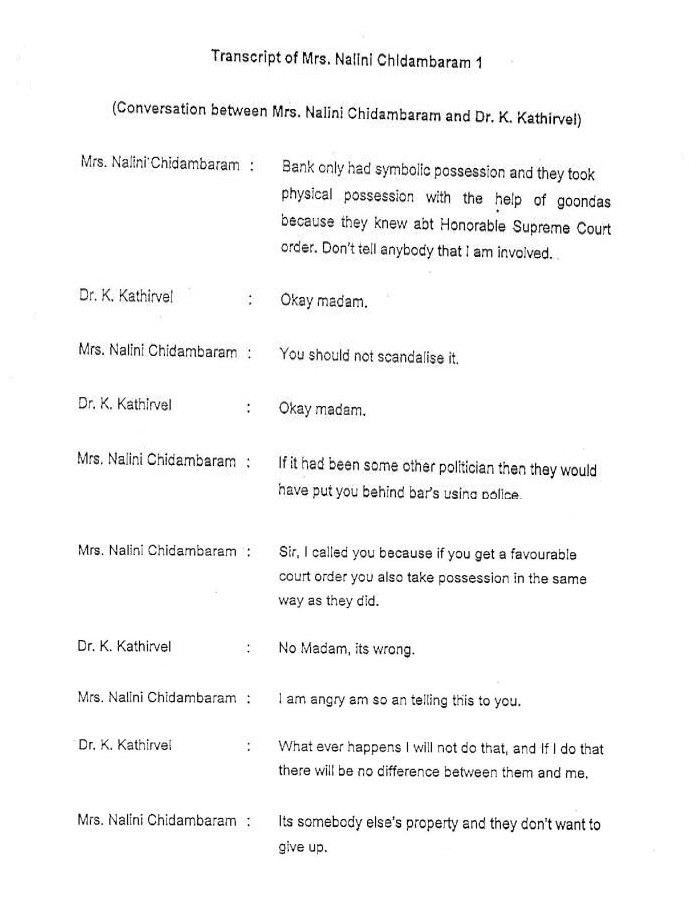
\includegraphics[height=4cm]{figures/conversation}};
        \node (b) at(3,0) {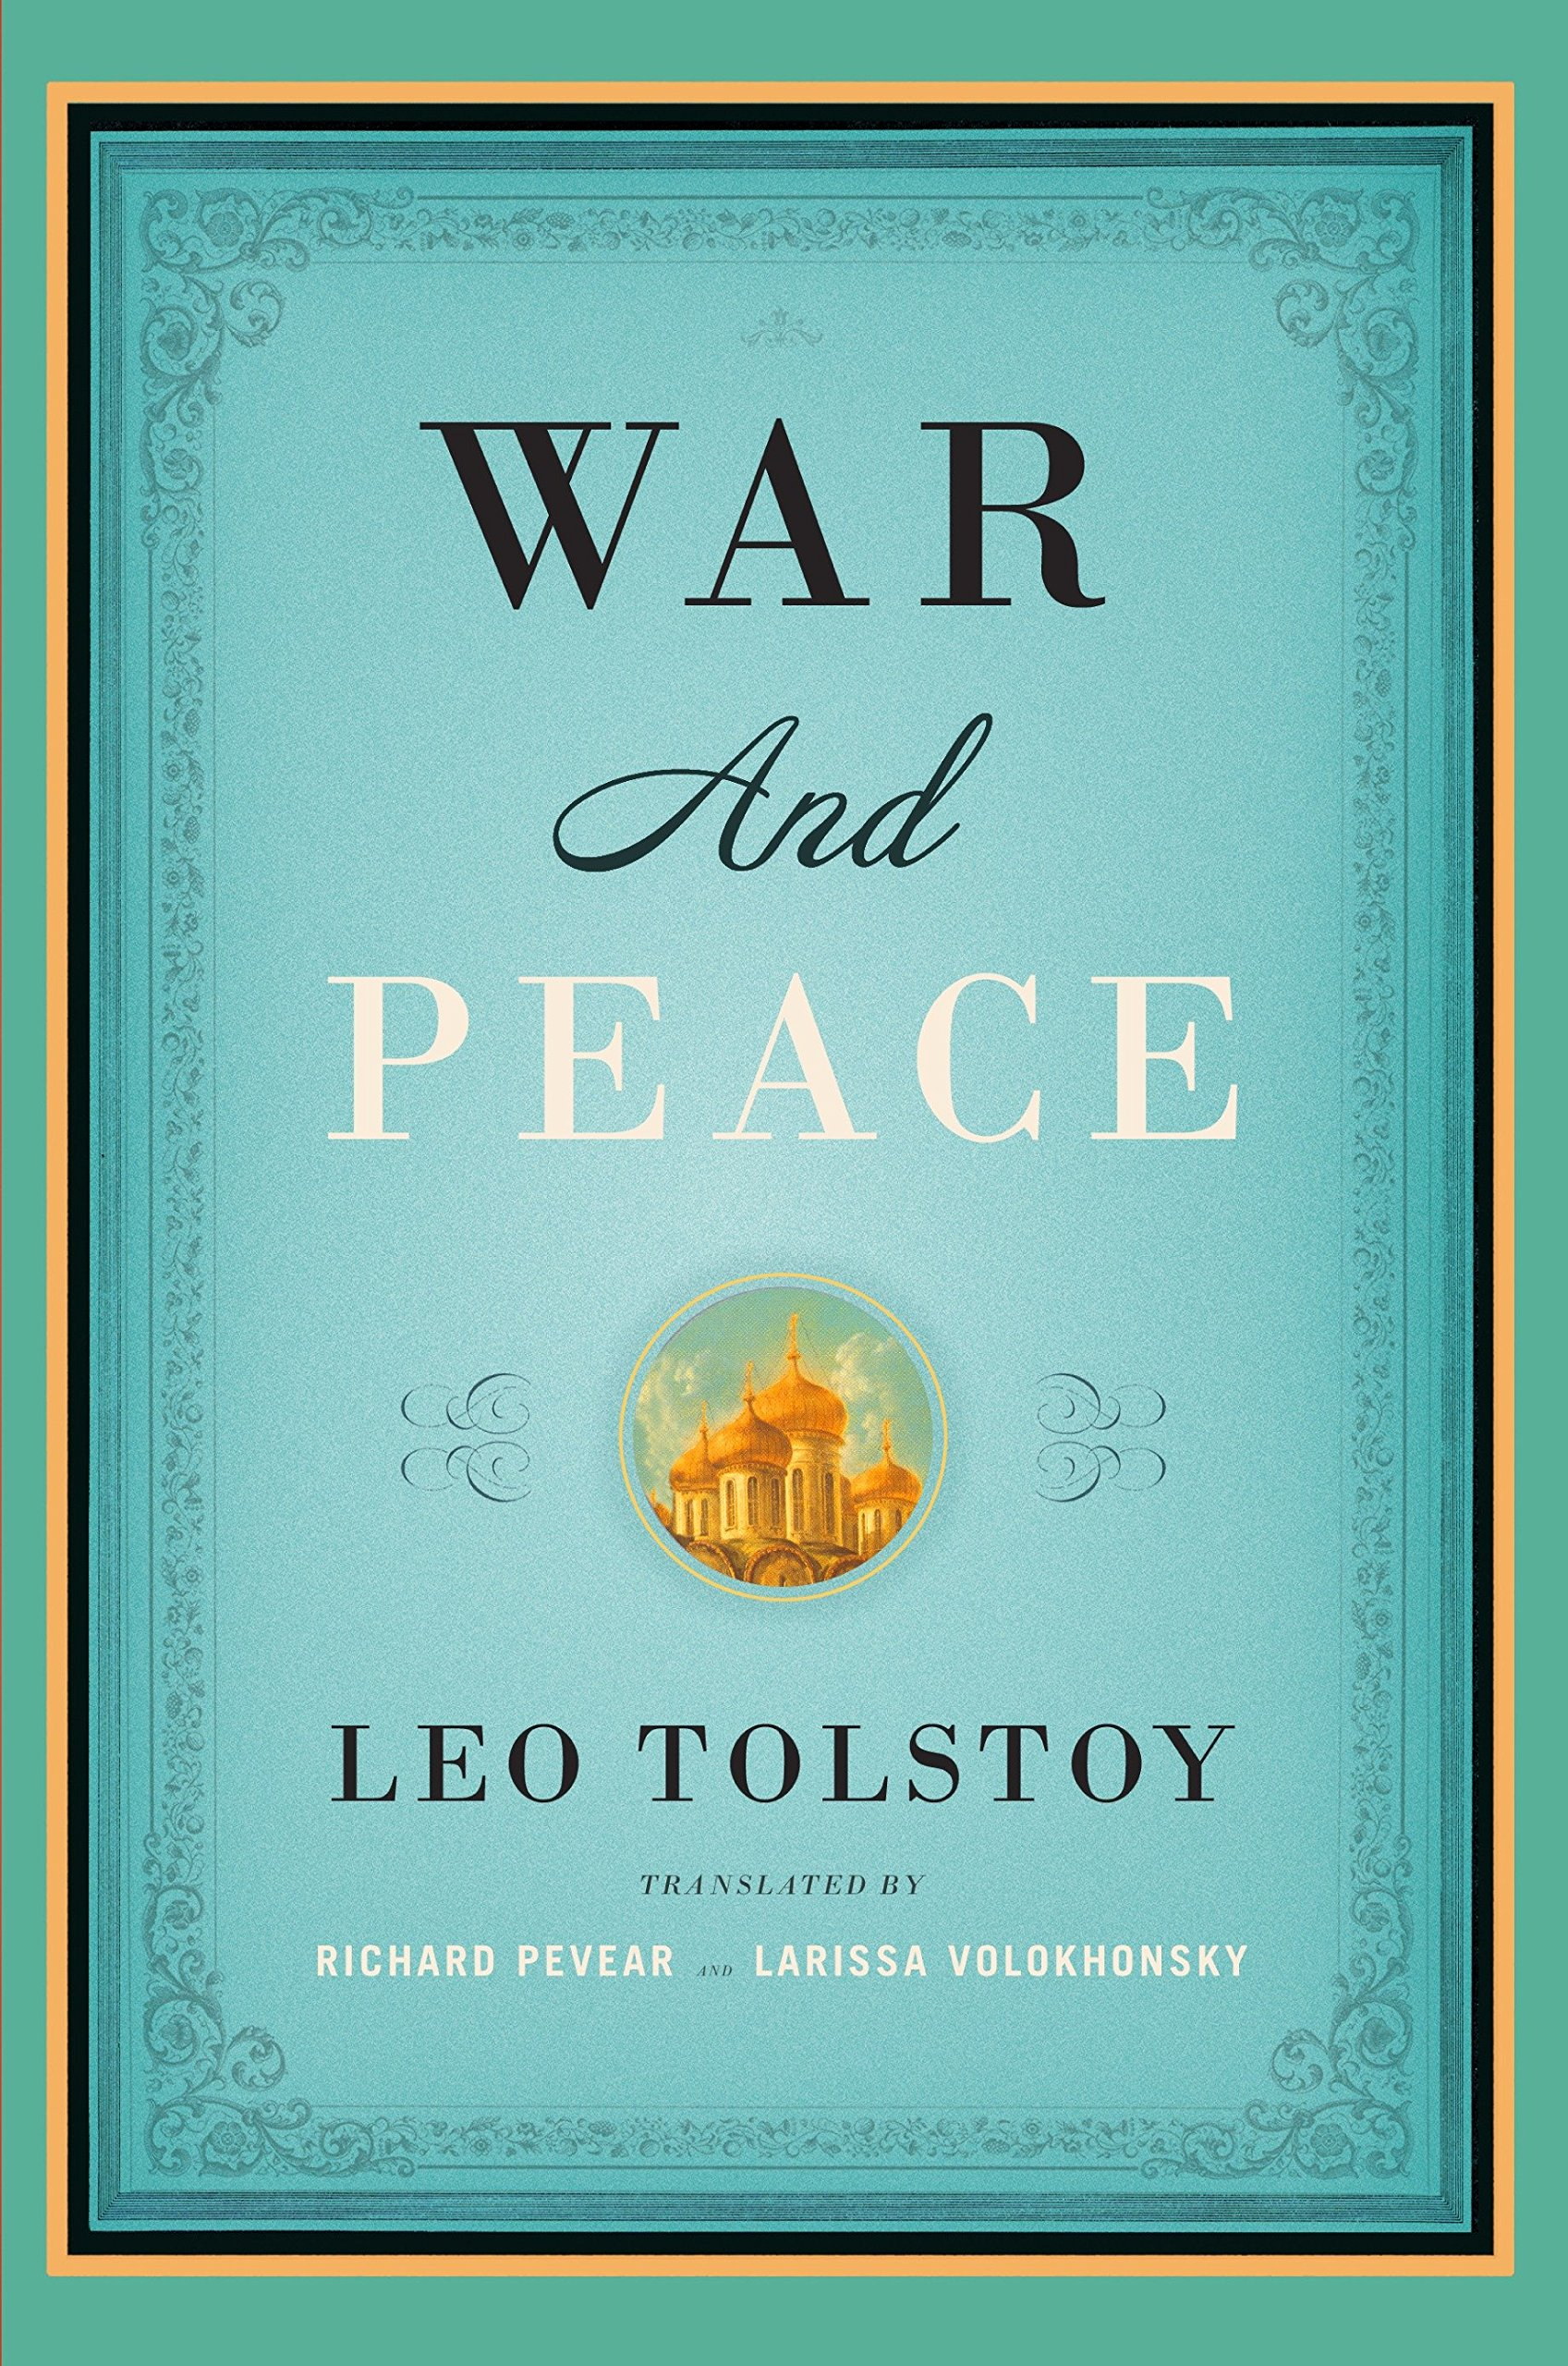
\includegraphics[height=4cm]{figures/novel}};
        \node (c) at(6,0) {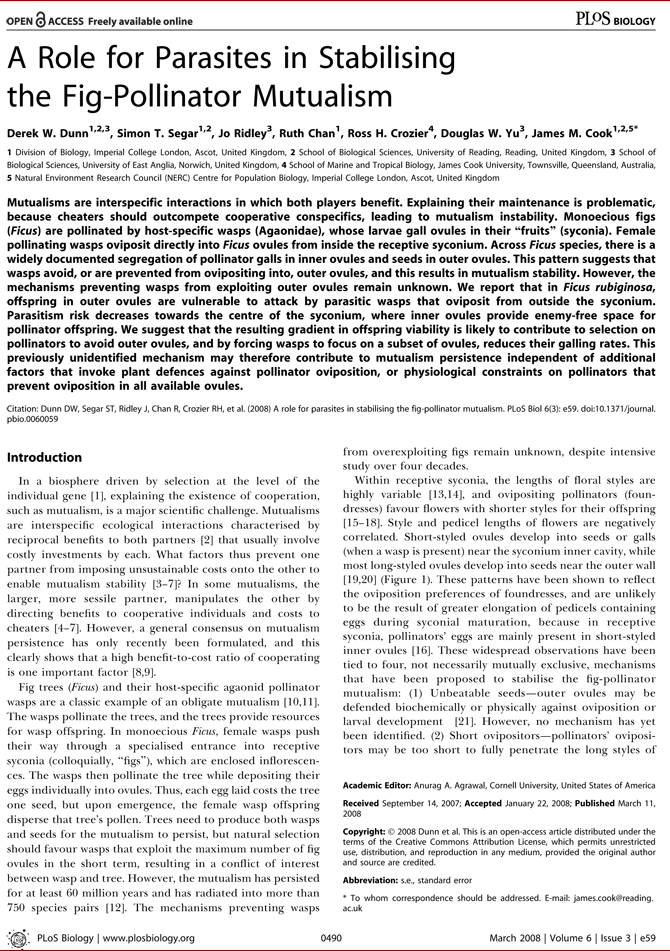
\includegraphics[height=4cm]{figures/paper}};
    \end{tikzpicture}
    \end{center}
\end{frame}

\begin{frame}
    {Beyond individual sentences: grounding}
    Connect language to the world

    \begin{center}
        \nl{Can you bring me an apple?}
        \begin{figure}
        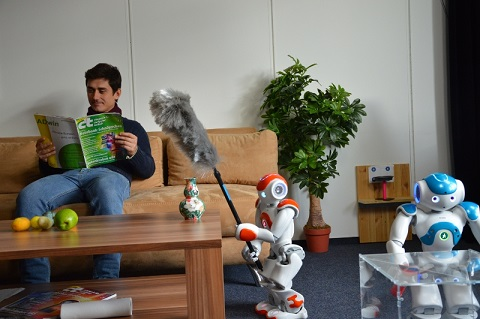
\includegraphics[height=4cm]{figures/robot-home}
        \end{figure}
    \end{center}
\end{frame}

\begin{frame}
    {Project}
    \begin{itemize}
        \itemsep1em
        \item Related to NLP (doesn't have to be in the scope of this course)
        \item New algorithms or models for existing problems
        \item Novel applications of NLP techniques 
        \item Analysis of well-known approaches that leads to new insight
        \item Overall rule: should increase our knowledge in some way
    \end{itemize}
\end{frame}

\end{document}
